\section{Running the App}
The app was then tested by visiting the \textit{sign in} page of static website. A user was registered and then redirect to the verification page. As expected, an email was received containing a verification code.


\begin{figure}[H]
  \caption{Verification Email}
  \centering
  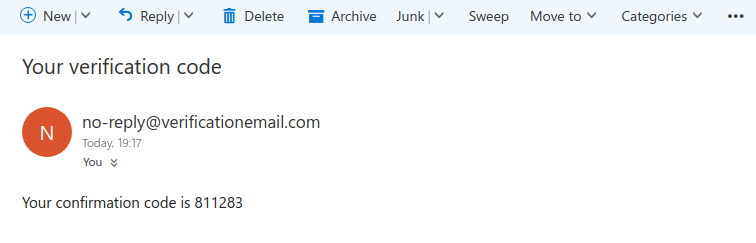
\includegraphics[width=0.75\textwidth,keepaspectratio]{verification-email}
  \label{fig:email}
\end{figure}

\noindent Once the user verified by entering the code, they were redirect to the main page of the app. Viewing the users on the AWS console Cognito page, dmeonstrated that user were successfully registering and verifying.

\begin{figure}[H]
  \caption{Users}
  \centering
  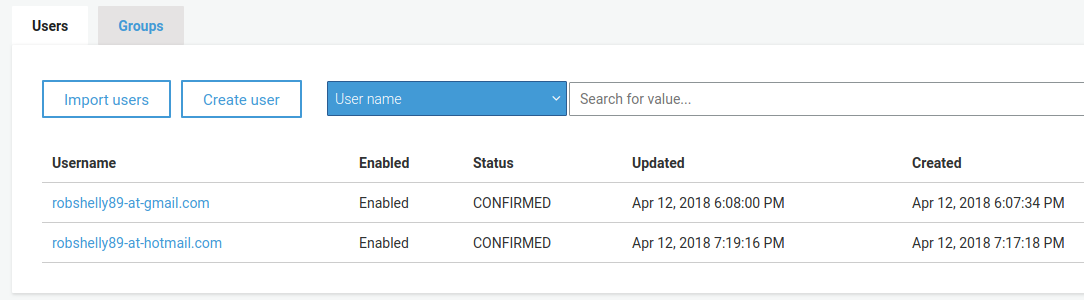
\includegraphics[width=\textwidth,keepaspectratio]{users}
  \label{fig:users}
\end{figure}

\noindent Finally the main aspect of the serverless web app could be tested by entering a location on the map and choosing \textit{Request a Unicorn}. This returned a response to the user containing a Unicorn and some details, shown if \autoref{fig:result}. The web also demonstrated that the user has successfully received a JSON web token, verifying that the user authentication is working. 

\begin{figure}[H]
  \caption{Successful Serverless Web App}
  \centering
  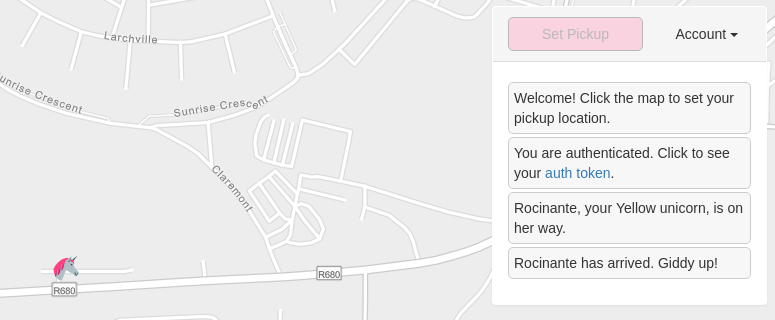
\includegraphics[width=\textwidth,keepaspectratio]{results}
  \label{fig:results}
\end{figure}

\noindent Viewing the \textit{Rides} table on DynamoDB also verifies that the Lambda backend is functioning correctly as the rides and relevant information have been entered into the table.

\begin{figure}[H]
  \caption{Rides Added to Backend Database}
  \centering
  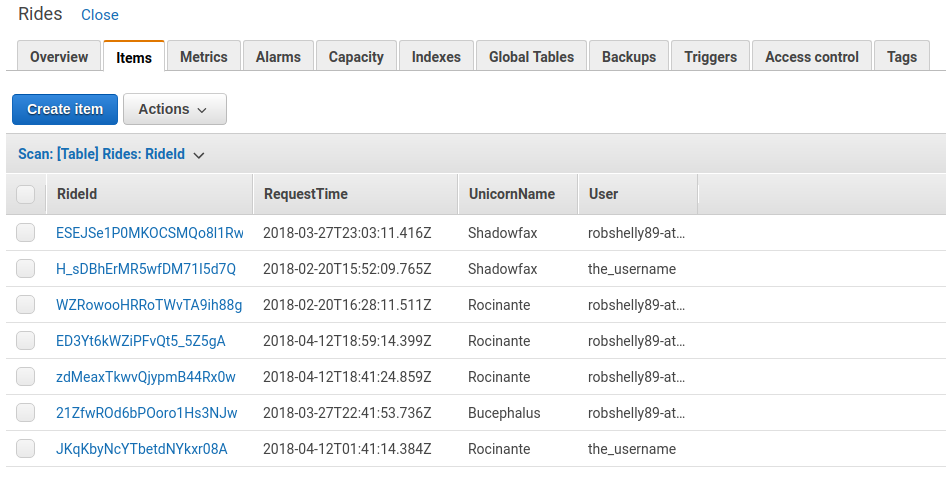
\includegraphics[width=\textwidth,keepaspectratio]{rides}
  \label{fig:rides}
\end{figure}
